\documentclass[UTF8]{ctexart}
\usepackage[a4paper, margin=1in]{geometry}
\usepackage{amsmath}
\usepackage{blkarray}
\usepackage{graphicx}
\usepackage{tikz}
\usetikzlibrary{matrix, positioning}
\usepackage{booktabs}

\title{从离散方程到分块矩阵的完整演变过程}
\author{数值传热学分析}
\date{\today}

\begin{document}

\maketitle

\section{问题描述}
考虑一个简单的2×2网格系统(总4个节点),展示二维热传导方程隐式离散如何形成原始矩阵,再如何演变为分块矩阵。

\subsection{网格点标记}
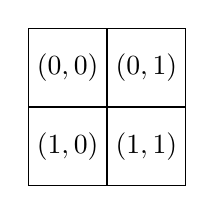
\begin{tikzpicture}
\draw[step=1,black,thin] (0,0) grid (2,2);
\node at (0.5,1.5) {$(0,0)$};
\node at (1.5,1.5) {$(0,1)$};
\node at (0.5,0.5) {$(1,0)$};
\node at (1.5,0.5) {$(1,1)$};
\end{tikzpicture}

\subsection{行优先索引}
\begin{tabular}{c|c|c}
节点 $(i,j)$ & 索引 $k$ & 含义 \\ \hline
$(0,0)$ & 0 & 左上 \\
$(0,1)$ & 1 & 右上 \\
$(1,0)$ & 2 & 左下 \\
$(1,1)$ & 3 & 右下 \\
\end{tabular}

\section{离散方程}
通用离散方程为:
$$
-r_x T_{i-1,j} - r_y T_{i,j-1} + (1 + 2r_x + 2r_y) T_{i,j} - r_x T_{i+1,j} - r_y T_{i,j+1} = T_{i,j}^n
$$

其中$d = 1 + 2r_x + 2r_y$。

对4个节点分别写方程:

\subsection{节点(0,0)方程}
$$
d T_{0,0} - r_x T_{1,0} - r_y T_{0,1} = T_{0,0}^n + r_x T_{-1,0} + r_y T_{0,-1}
$$
边界项移到右侧

\subsection{节点(0,1)方程}
$$
d T_{0,1} - r_x T_{1,1} - r_y T_{0,0} = T_{0,1}^n + r_x T_{-1,1} + r_y T_{0,2}
$$

\subsection{节点(1,0)方程}
$$
d T_{1,0} - r_x T_{0,0} - r_y T_{1,1} = T_{1,0}^n + r_x T_{2,0} + r_y T_{1,-1}
$$

\subsection{节点(1,1)方程}
$$
d T_{1,1} - r_x T_{0,1} - r_y T_{1,0} = T_{1,1}^n + r_x T_{2,1} + r_y T_{1,2}
$$

\section{原始矩阵形式}
将方程组织成线性系统 $\mathbf{A}\mathbf{T} = \mathbf{b}$:

$$
\mathbf{A} =
\begin{blockarray}{cccccc}
& k=0 & k=1 & k=2 & k=3 \\
\begin{block}{c(cccc)c}
k=0: & d & -r_y & -r_x & 0 & \leftarrow (0,0) \\
k=1: & -r_y & d & 0 & -r_x & \leftarrow (0,1) \\
k=2: & -r_x & 0 & d & -r_y & \leftarrow (1,0) \\
k=3: & 0 & -r_x & -r_y & d & \leftarrow (1,1) \\
\end{block}
\end{blockarray}
$$

$$
\mathbf{b} =
\begin{bmatrix}
T_{0,0}^n + r_x T_{-1,0} + r_y T_{0,-1} \\
T_{0,1}^n + r_x T_{-1,1} + r_y T_{0,2} \\
T_{1,0}^n + r_x T_{2,0} + r_y T_{1,-1} \\
T_{1,1}^n + r_x T_{2,1} + r_y T_{1,2} \\
\end{bmatrix}
$$

\section{分块矩阵演变}

\subsection{步骤1:识别网格行}
将节点按网格行分组:
\begin{itemize}
\item 第0行: 节点(0,0)和(0,1) → 索引0,1
\item 第1行: 节点(1,0)和(1,1) → 索引2,3
\end{itemize}

\subsection{步骤2:定义子矩阵块}

定义三个类型的子矩阵:
\begin{enumerate}
\item $B_i$: 第$i$行内部的耦合关系
\item $A_i$: 第$i$行与第$i-1$行的耦合
\item $C_i$: 第$i$行与第$i+1$行的耦合
\end{enumerate}

\subsection{步骤3:构建子矩阵}

\subsubsection{$B_0$ (第0行内部)}
$$
B_0 =
\begin{bmatrix}
d & -r_y \\
-r_y & d \\
\end{bmatrix}
$$

\subsubsection{$B_1$ (第1行内部)}
$$
B_1 =
\begin{bmatrix}
d & -r_y \\
-r_y & d \\
\end{bmatrix}
$$

\subsubsection{$A_1$ (第1行到第0行的耦合)}
$$
A_1 =
\begin{bmatrix}
-r_x & 0 \\
0 & -r_x \\
\end{bmatrix}
$$

\subsubsection{$C_0$ (第0行到第1行的耦合)}
$$
C_0 =
\begin{bmatrix}
-r_x & 0 \\
0 & -r_x \\
\end{bmatrix}
$$

\subsection{步骤4:组合分块矩阵}
$$
\mathbf{A} =
\begin{bmatrix}
B_0 & C_0 \\
A_1 & B_1 \\
\end{bmatrix}
=
\begin{bmatrix}
d & -r_y & -r_x & 0 \\
-r_y & d & 0 & -r_x \\
-r_x & 0 & d & -r_y \\
0 & -r_x & -r_y & d \\
\end{bmatrix}
$$

\section{一般情况推广}

对于$N_x \times N_y$网格,分块矩阵为:
$$
\mathbf{A} =
\begin{bmatrix}
B_0 & C_0 & 0 & \cdots & 0 \\
A_1 & B_1 & C_1 & \ddots & \vdots \\
0 & A_2 & B_2 & \ddots & 0 \\
\vdots & \ddots & \ddots & \ddots & C_{N_x-2} \\
0 & \cdots & 0 & A_{N_x-1} & B_{N_x-1} \\
\end{bmatrix}
$$

其中:
\begin{itemize}
\item $B_i$: $N_y \times N_y$ 三对角矩阵
\item $A_i$: $N_y \times N_y$ 对角矩阵
\item $C_i$: $N_y \times N_y$ 对角矩阵
\end{itemize}

\section{物理意义图解}

\begin{tikzpicture}[
    node distance=1.5cm,
    gridnode/.style={draw,circle,minimum size=1cm},
    matrixnode/.style={draw,rectangle,minimum size=0.7cm}
]

% 网格节点
\node[gridnode] (00) at (0,0) {0};
\node[gridnode,right=of 00] (01) {1};
\node[gridnode,below=of 00] (10) {2};
\node[gridnode,below=of 01] (11) {3};

% 网格内耦合
\draw[red,<->] (00) -- node[midway,above] {$-r_y$} (01);
\draw[red,<->] (10) -- node[midway,above] {$-r_y$} (11);

% 行间耦合
\draw[blue,<->] (00) -- node[midway,left] {$-r_x$} (10);
\draw[blue,<->] (01) -- node[midway,right] {$-r_x$} (11);

% 矩阵表示
\node[matrixnode] (m00) at (4,2) {d};
\node[matrixnode,right=of m00] (m01) {$-r_y$};
\node[matrixnode,right=of m01] (m02) {$-r_x$};
\node[matrixnode,right=of m02] (m03) {0};

\node[matrixnode,below=of m00] (m10) {$-r_y$};
\node[matrixnode,right=of m10] (m11) {d};
\node[matrixnode,right=of m11] (m12) {0};
\node[matrixnode,right=of m12] (m13) {$-r_x$};

\node[matrixnode,below=of m10] (m20) {$-r_x$};
\node[matrixnode,right=of m20] (m21) {0};
\node[matrixnode,right=of m21] (m22) {d};
\node[matrixnode,right=of m22] (m23) {$-r_y$};

\node[matrixnode,below=of m20] (m30) {0};
\node[matrixnode,right=of m30] (m31) {$-r_x$};
\node[matrixnode,right=of m31] (m32) {$-r_y$};
\node[matrixnode,right=of m32] (m33) {d};

% 连接关系
\draw[->] (01) to [out=0,in=90] (m01);
\draw[->] (10) to [out=0,in=90] (m20);
\draw[->] (11) to [out=0,in=270] (m33);
\end{tikzpicture}

\begin{itemize}
\item \textcolor{red}{红色}连接:行内耦合 ($-r_y$),反映在$B_i$矩阵的非对角线上
\item \textcolor{blue}{蓝色}连接:行间耦合 ($-r_x$),反映在$A_i$和$C_i$矩阵的对角线上
\item 网格中的每个连接点直接对应矩阵中的非零元素位置
\end{itemize}

\section{结论}
通过这个分析,我们清晰地展示了:
1. 如何从离散方程得到原始矩阵
2. 如何识别网格的物理结构组织矩阵块
3. 子矩阵块 $B_i$, $A_i$, $C_i$ 的物理意义
4. 如何将原始矩阵重组为块状结构

分块矩阵不是人为创造,而是对热传导物理耦合关系的自然数学表达。这种表达方式:
\begin{itemize}
\item 保持矩阵的原始数学特性
\item 反映物理系统的空间结构
\item 便于高效存储和求解
\item 为复杂边界条件的处理提供框架
\end{itemize}

\end{document}